\chapter{Анализ предметной области}

Прежде чем приступить к обзору и анализу существующих средств сетевого мониторинга ядра Linux, необходимо определить что подразумевается под сетевым мониторингом ядра Linux

\section{Ядро Linux}
Ядро Linux --- это основной внутренний компонент операционной системы Linux, отвечающие за распределением системными ресурсами, управление аппаратным обеспечением и обеспечение взаимодействие приложения с аппаратным обеспечением~\cite{kernel_linux_robert}.

В Linux системах ядро является монолитным с модульной конструкцией, которое реализовано в виде одного большого процесса, выполняющий в одном адресном пространстве.
Такие ядра обычно хранятся на диске в виде одного большого статического бинарного файла.
Все службы ядра находятся и выполняются в одном большом адресном пространстве ядра.
Взаимодействия в ядре осуществляются очень просто, потому что все, что выполняется в режиме ядра, выполняется в одном адресном пространстве.
В отличие от микроядра, который разделяет службы ядра на несколько процессов, называемыми серверами.
Ядро может вызывать функции непосредственно, как это делают пользовательские приложения.

Главным задачами ядра в первую очередь является:
\begin{enumerate}
	\item обеспечение среды выполнения для программ в операционной системе;
	\item взаимодействие с аппаратными компонентами и обслуживание их низкоуровневые элементы.
\end{enumerate}

В современных системах с устройствами управления защищенной памятью ядро обычно занимает привилегированное положение по отношению к пользовательским программам. Это включает доступ ко всем областям защищенной памяти и полный доступ к аппаратному обеспечению. Системные переменные (system state) и область памяти, в которой находится ядро, вместе называются пространством ядра (kernel-space), или привилегированным режимом, или также называется <<режим ядра>>. Соответственно, пользовательские программы выполняются в пространствах задач (user-space), или в <<пользовательском режиме>>.

\section{Подсистемы ядра}
Ядро Linux разделяется на ряд подсистем, рисунок \ref{img:arch_linux}, как на высоком, так и на низких уровнях. Такое разделение позволяет упростить разработку ядра и сделать его более гибким.
Каждая подсистема выполняет реализует свой функционал, такие как управление памятью, управление и взаимодействие процессов, файловая система, сетевые стек, которое используется другими подсистемами.  

\begin{figure}[h!]
	\centering
	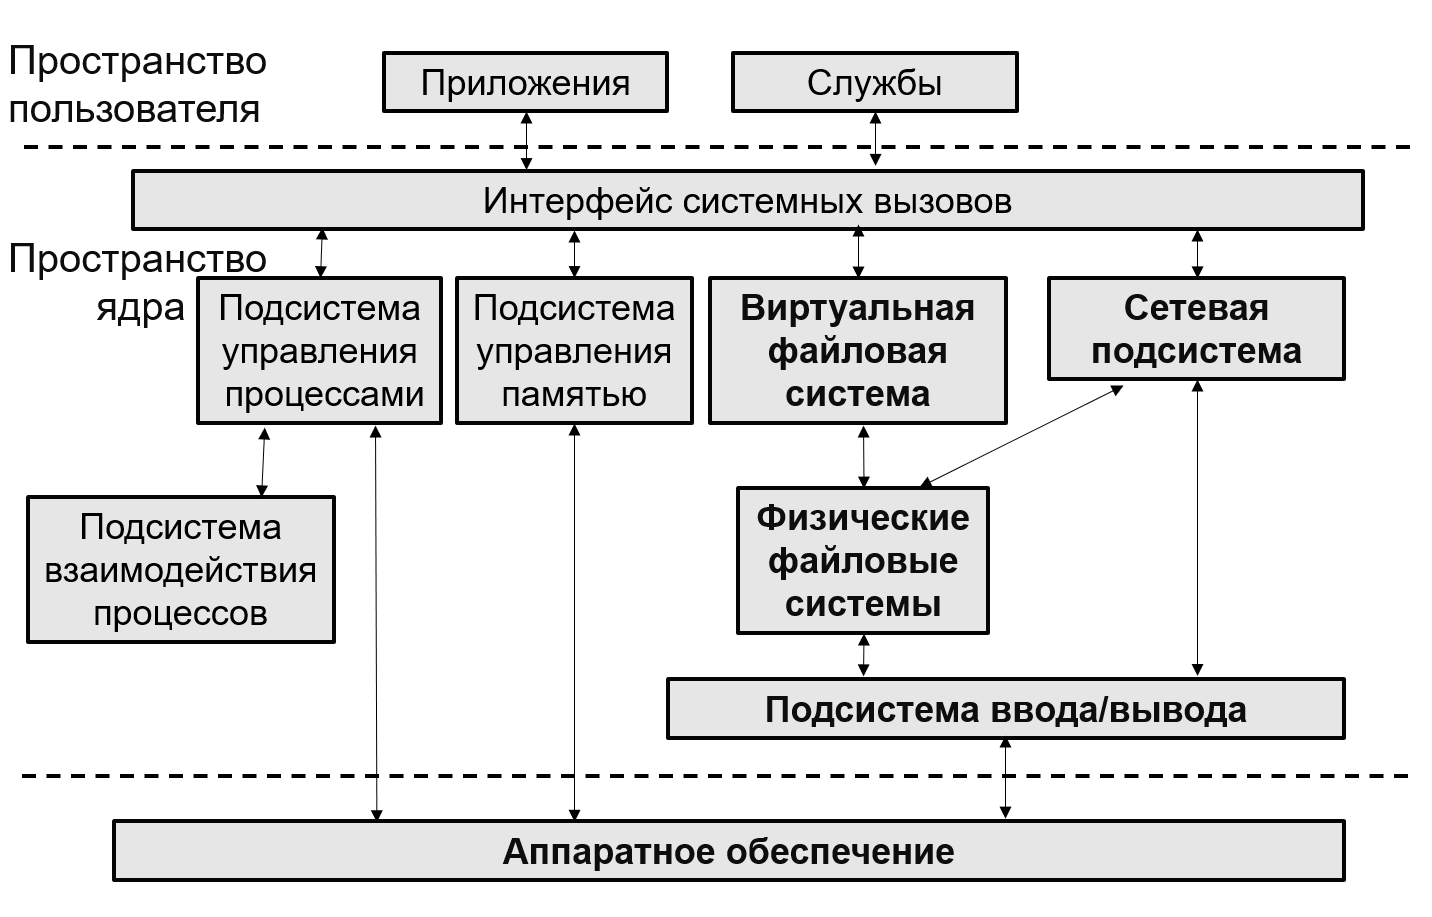
\includegraphics[height=0.4\textheight]{img/arch_linux} % height
	\caption{Общая архитектура Linux}
	\label{img:arch_linux}
\end{figure}

\clearpage

\section{Сетевая подсистема ядра}

Сетевая подсистема ядра Linux \cite{moduls_kernel_linux, linux_network_internals} обеспечивает взаимодействие процессов, выполняющихся на разных узлах сети, то есть дает возможность сетевого взаимодействия между приложениями .

Сетевая подсистема ядра Linux реализует следующий функционал:
\begin{itemize}
	\item поддержку взаимодействия процессов с помощью механизмов сокетов (sockets);
	\item реализацию стеков сетевых протоколов (TCP/IP, UDP/IP, IPX/SPX и другие);
	\item поддержку сетевых интерфейсов;
	\item обеспечение маршрутизации пакетов (routing);
	\item обеспечение фильтрации пакетов (netfilter).
\end{itemize}

Взаимодействие сетевой подсистемы с другими подсистема ядра показана на рисунке \ref{img:arch_linux}.

\subsection{Многоуровневая модель}

Для решения задачи сетевых взаимодействий применяется многоуровневый иерархический подход, заключающийся в разбиении процесса коммуникации на набор уровней с четко определенными способами взаимодействия уровней на одном узле и на соседних узлах. 
Таким образом в подсистеме существует сетевой стек, который является производной стека BSD.
Сетевой стек хорошо оснащен добротным набором интерфейсов, которые варьируются от протоколо-независимых (protocol agnostic), таких как интерфейс уровня общих сокетов или уровня устройств, до специальных интерфейсов конкретных сетевых протоколов. 
Уровень сокетов представляет собой стандартный API к сетевой подсистеме. 
Он предоставляет пользовательский интерфейс к различным сетевым протоколам. 
Уровень сокетов реализует стандартизованный способ управления соединениями и передачи данных между конечными точками, от доступа к <<чистым>> кадрам данных и блокам данных протокола IP/PDU, и до протоколов TCP/UDP.

В то время как работа в сети отсылается к модели сетевого взаимодействия по OSI, сетевой стек в Linux использует модель TCP/IP \cite{tcpip_craig, tcpip_lora}, включающая в себя 4 уровня:
\begin{enumerate}
	\item уровень сетевых интерфейсов (канальный уровень) относится к драйверам устройств, обеспечивающим доступ к физическому уровню, который может состоять из многочисленных сред, таких как последовательные каналы или устройства Ethernet, описываются как сетевые интерфейсы;
	\item уровень межсетевого взаимодействия (сетевой уровень) обеспечивает работу базовой
	службы доставки пакетов по назначению;
	\item транспортный уровень обеспечивает надежную доставку данных со сквозным обнаружением и устранением ошибок;
	\item прикладной уровень отвечает за взаимодействие с приложениями и процессами на хостах, также определяются пользовательские интерфейсы процесса или приложения, наблюдается работа протоколов и служб --- FTP, Telnet и другие. 
\end{enumerate}
Сетевая модель TCP/IP условно согласуется с моделью OSI, включающая в себя 7 уровней:
\begin{enumerate}
	\item физический уровень;
	\item канальный уровень;
	\item сетевой уровень;
	\item транспортный;
	\item сеансовый уровень;
	\item представительский уровень;
	\item прикладной уровень.
\end{enumerate}

\clearpage

На рисунке \ref{img:protocol} показано как модели  TCP/IP и OSI пересекаются между собой.
\begin{figure}[h!]
	\centering
	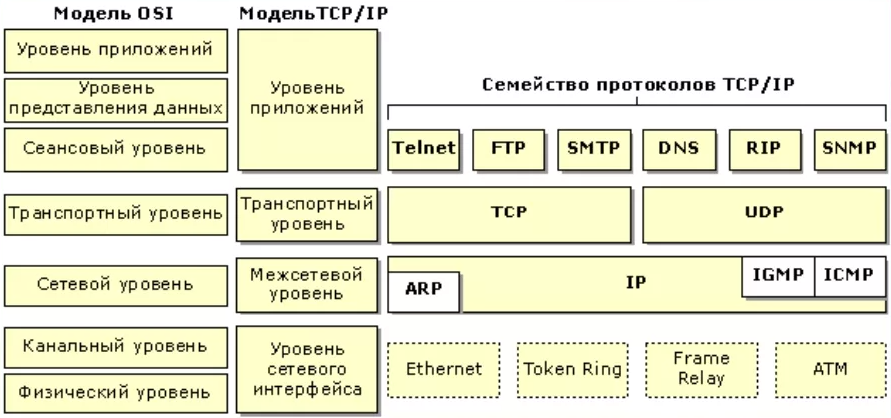
\includegraphics[height=0.3\textheight]{img/protocol}
	\caption{Модель OSI и TCP/IP}
	\label{img:protocol}
\end{figure}

\subsection{Сетевой интерфейс}

Сетевые интерфейсы являются основой сетевой подсистемы, иначе говоря абстракцией, используемые для представления связи устройств сети с протоколом TCP/IP и передачи данных через некоторые линии связи.
Основными устройствами, позволяющими организовывать взаимодействие по сети, являются сетевые адаптеры (Ethernet-карты).

Интерфейс имеет набор параметров, большинство которых относятся к сетевому уровню (IP-адрес, маска сети и т.п.).
Важным параметром сетевого интерфейса является аппаратный адрес. 
В Ethernet аппаратный адрес называется MAC-адрес и состоит из шести байтов, которые принято записывать в шестнадцатеричной системе исчисления и разделять двоеточиями.

\textbf{TODO: возможно включить подробности}

\section{Сетевой мониторинг ядра}

Сетевой мониторинг ядра Linux --- это контролирование пакетов и нахождение наличие ошибок сетевых интерфейсов сетевой подсистемы, что относится вмешательством в работу подсистемы и ее сетевого стека.

\textbf{TODO: подробнее описать ПОПРАВИТЬ}
Часто мониторинг сетевой подсистемы операционной системы заканчивается на счетчиках пакетов, октетов и ошибок сетевых интерфейсах. Но это только 2й уровень модели OSI!
С одной стороны большинство проблем с сетью возникают как раз на физическом и канальном уровнях, но с другой стороны приложения, работающие с сетью оперируют на уровне TCP сессий и не видят, что происходит на более низких уровнях.

